\newpage
\restoregeometry
\section{Implementierung}
\subsection{Softwarestack}
Die prototypische Entwicklung eines Rich Data Interface für Copernicus-Daten erfolgte im Rahmen dieser Arbeit mit der Programmiersprache Python.
Diese ist nicht nur aufgrund ihrer Einfachheit vorteilhaft, sondern erlaubt auch den Zugriff auf eine große Zahl von Packages für die unterschiedlichsten 
Anwendungsfälle. Weite Teile des Rich Data Interface wurden mithilfe des \verb|flask|-Frameworks umgesetzt. Dieses erlaubt das schnelle Entwickeln einer leichtgewichtigen API.  
Neben Python Standard-Bibliotheken finden nur wenige zusätzliche Packages Verwendung. Um zu Anfragen passende Sentinel-1 Datensätze aus dem 
Copernicus Open Access Hub zu finden kommt das Package \verb|sentinelsat| zum Einsatz. Das Herunterladen der Sentinel-1 Datensätze erfolgt ebenfalls mit diesem Package. 
Die Vorprozessierung der Sentinel-1 Datensätze werden mit dem Package \verb|snappy| durchgeführt. 
Dieses ist ein Wrapper für die Sentinel Application Platform (SNAP), welche im Rahmen des Copernicus-Programmes kostenlos zur Verfügung 
gestellt wird. Mithilfe von \verb|snappy| lassen sich die Funktionen der Sentinel-1 Toolbox der SNAP in Python verwenden. 
Statistische Auswertungen der Radarbilder werden mit dem Package \verb|skimage| durchgeführt. 
Für das Zuschneiden und mathematische Kombinieren der Radarbilder kommen das \verb|osgeo| Package und das Modul \verb|gdal| zum Einsatz.
Die Versionierung erfolgt mit Git und der Plattform GitHub. 

\subsection{Struktur}
Die Anwendung ist in vier Python-Scripte aufgeteilt. Im \verb|api.py| Script ist die API der Anwendung definiert. 
Die API setzt die Requirements-Classes Core, OGC Process Description, JSON, HTML, OpenAPI 3.0, Job List und Dismiss um.
Die geordnete Abarbeitung der angelegten Jobs wird vom Script \verb|processing.py| nach dem Modell der Queue gesteuert. 
Dies bedeutet, dass zeitgleich nur ein Job ausgeführt wird. Nach dessen Beendigung wird der älteste angelegte Job gewählt und bearbeitet.
Die eigentlichen Prozesse sowie 
Hilfsfunktionen befinden sich im \verb|utils.py| Script. Dazu zählen auch die eigentlichen Prozesse sowie Parser für 
ihre Eingabedaten. Das \verb|test.py| Script kann dazu genutzt werden, um die Stabilität und Standardkonformität der API zu testen und enthält den Test-Suit.

Diese Scripte verwalten Dateien in einem einfachen Verzeichnissystem. Templates für statische Ressourcen befinden sich im \emph{Templates}-Verzeichnis. In den Unterverzeichnissen 
\emph{HTML} und \emph{JSON} befinden sich die Repräsentationen von Ressourcen als \verb|.html| und \verb|.json|-Dateien.  
Das \emph{Processes}-Unterverzeichnis enthält die Beschreibungen der von der Anwendung angebotenen Prozesse. 
Die Anwendung erlaubt das persistente Hinterlegen von Sentinel-1 Datensätzen. Diese Datensätze können im \emph{Data}-Verzeichnis 
abgelegt werden. Jeder Sentinel-1 Datensatz enthält eine \verb|.kml|-Datei, welche Metadaten zum Datensatz enthält. Diese werden im \emph{Coverage}-Unterverzeichnis abgelegt. 
Jeder angelegte Job, also jede auszuführende Instanz eines Prozesses erhält ein einzigartiges Verzeichnis innerhalb des Verzeichnisses \emph{Jobs}. In diesem 
Verzeichnis befinden sich eine \verb|status.json| und eine \verb|job.json| sowie weitere für die Bearbeitung des Jobs benötigte Dateien. 
Neben diesen Dateien enthält jedes \emph{Job}-Verzeichnis ein \emph{Results}-Unterverzeichnis in dem die Ergebnisse des jeweiligen Jobs abgelegt werden (siehe Abbildung \ref{structure}) \cite{code}.

\begin{figure}[H]
    \centering
    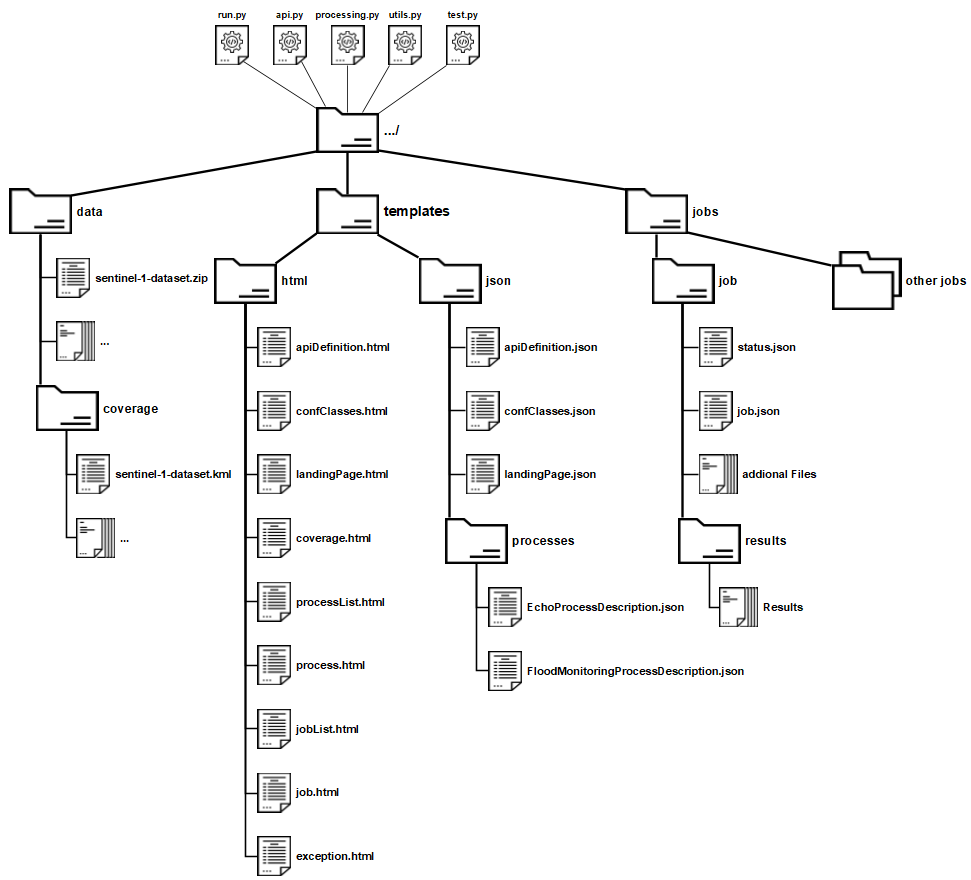
\includegraphics[width=\textwidth]{Bilder/folders.png}
    \caption{Struktur der prototypischen Implementierung \cite{code}}
    \label{structure}
\end{figure}

\subsection{Ressourcen}
Ressourcen sind die über die Endpoints der API bereitgestellten Informationen und Dateien. Sie können in unterschiedlichen Repräsentationen vorliegen. 
Die Ressourcen werden vom OGC API - Processes - Part 1: Core Standard mittels \verb|.yaml|-Schemadateien beschrieben. 
Diese definieren neben den Bezeichnungen für Attribute auch ihre Datentypen und ob diese optional sind oder nicht. 
Die meisten angebotenen Ressourcen können um Media-Type \verb|text/html| oder im Media-Type \verb|application/json| angefragt werden. 
Um aus diesen Dateien einen Response zu generieren, werden \verb|.html|-Dateien zuvor mit der Methode \verb|render_template()|, welcher auch 
dynamische Inhalte übergeben werden können, gerendert, während \verb|.json|-Dateien zunächst geladen und anschließend 
mit der Methode \verb|jsonify()| bearbeitet werden. Beide genannten Methoden
geben ein Response-Objekt zurück, welches zusammen mit Headern und einem HTTP-Statuscode versandt werden kann.
Die meisten Ressourcen enthalten zudem eine Verknüpfung zu sich selbst mit der Relation \verb|self| und gegebenenfalls eine Verknüpfung 
zur Ressource im jeweils anderen Media-Type mit der Relation \verb|alternate|.

\subsection{Encodings}
In der Requirements Class JSON wird definiert welche Ressourcen im \verb|JSON|-Format, also dem Media-Type \verb|application/json|, 
angefragt werden können. Dazu gehören alle Responses der 
Endpunkte API Landing Page, API-Definition, Conformance Deklaration, Process List, Prozess Description, Prozess Execution und Job Status, welche mit dem 
HTTP-Statuscode 200 versandt werden. Da die prototypische Implementierung auch die Endpunkte Job List und Coverage bereitstellt, können die korrespondierenden
Ressourcen auch im Media-Type \verb|application/json| angefragt werden.\\

In der Requirements Class HTML werden analog zur Requirements Class JSON jene Ressourcen definiert, welche im \verb|HTML|-Format, also im Media-Type \verb|text/html| 
angefragt werden können. Jedoch entfällt in dieser Requirements Class die Einschränkung auf bestimmte Endpunkte und alle Responses, 
welche mit dem HTTP-Statuscode 200 versandt werden, müssen den Media-Type \verb|text/html| unterstützen.
Stellen Endpoints ihre Ressourcen sowohl den Media-Type \verb|application/json| als auch \verb|text/html| zur Verfügung, so können Nutzer*innen diesen über den optionalen Parameter
\verb|f| spezifizieren. Wird kein Media-Type über diesen Parameter spezifiziert, so wird standardmäßig der Media-Type \verb|text/html| verwendet.

\subsection{Konfiguration der HTTP Version}
Die Umsetzung des Requirements HTTP 1.1 aus der Requirements Class Core verlangt, dass die API exklusiv das HTTP 1.1 unterstützt. 
Das \verb|flask|-Framework nutzt standardmäßig das HTTP 1.0. Teil des Frameworks ist die WSGI-Bibliothek \verb|Werkzeug|, welche
das Implementieren von Webanwendungen erlaubt. Um die verwendete HTTP-Version von 1.0 auf 1.1 umzustellen, müssen Variablen 
in \verb|Werkzeug| angepasst werden. Nach dem Import der Module \verb|WSGIRequestHandler| und \verb|BaseWSGIServer| wurde in beiden die 
Version des HTTP Protokolls durch Änderung von Variablen angepasst \cite{code}. 
In diesem Requirement werden zudem alle HTTP-Statuscodes gelistet, die Nutzer*innen von einer standardkonformen Implementierung mindestens erwarten können. 
Der Standard erlaubt die Nutzung weiterer HTTP-Statuscodes \cite{ogc_api_processes_core}.
 
\begin{table}[H]
    \caption{Vorgesehene HTTP-Statuscodes \cite{ogc_api_processes_core}}
    \centering
    \begin{tabular}{c c} 
        HTTP-Statuscode & Bedeutung\\ 
        \hline
        200 & Ok\\
        201 & Created\\
        204 & No Content\\
        400 & Bad Request\\
        401 & Unauthorized\\
        403 & Forbidden\\
        404 & Not Found\\
        405 & Method Not Allowed\\
        406 & Not Acceptable\\
        410 & Gone\\
        429 & Too Many Requests\\
        500 & Internal Server Error\\
        501 & Not Implemented\\
    \end{tabular}\label{httpcodes}
\end{table}

Zusätzlich enthalten die meisten Responses einen \verb|link|-Header,
welcher eine Verknüpfung mit der Relation \verb|self| enthält. Zusätzlich ist ein \verb|resource|-Header Teil eines Responses. Dieser 
identifiziert die angefragte Ressource zusätzlich.
%Alle erfolgreichen Anfragen, welche eine Resource liefern, werden mit dem HTTP-Statuscode 200 beantwortet. Die Verwendung nicht zulässiger HTTP-Methoden resultieren 
%in Antworten mit dem Status-Code 405 während Anfragen für nicht unterstütze Media-Types mit dem Status-Code 406 beantwortet werden. Kommt es zu Fehlern bei der Ausführung 
%des Programmcodes antwortet die Anwendung mit dem HTTP-Statuscode 500. Werden durch eine Anfrage Ressourcen neu erzeugt oder nicht gefunden antwortet die Anwendung mit 
%den HTTP-Statuscodes 201 beziehungsweise 404. 

\subsection{Endpoints der API}
\subsubsection{API Landig Page Endpoint}
Der API Landing Page Endpoint kann über den nachstehendem URL angefragt werden und liefert als Ressource die 
API Landing Page. 
\begin{center}
\begin{BVerbatim}
    http://HOST:PORT/?f=<MEDIA-TYPE>
\end{BVerbatim}
\end{center}
Der API Landing Page Endpoint ist Teil der Requirements Class Core. Die einzig zulässige HTTP-Methode für diesen Endpoint ist die HTTP-Get Methode.
Die API Landing Page kann als Eintrittspunkt zu allen anderen Funktionalitäten der Anwendung bezeichnet werden. Sie enthält Verknüpfungen zu den Endpoints, 
API Landing Page, API-Definition, Conformance, Process List, Process Description, Job List und Coverage.
Die API Landing Page kann in den Media-Types \verb|text/html| und \verb|application/json| abgerufen werden. 
Ein an den API Landing Page Endpoint gerichteter Request wird zunächst auf die verwendetet HTTP-Methode hin überprüft. Handelt es sich nicht um die HTTP-Get 
Methode wird der HTTP-Statuscode 405 als Response versandt. Im nächsten Schritt erfolgt die Prüfung des angefragten Media-Types. Enthält der Parameter \verb|f|
einen nicht unterstützten Media-Type wird als Response der HTTP-Statuscode 406 versandt. Wird der Media-Type nicht spezifiziert oder
\verb|text/html| angefragt wird die \verb|landingPage.html| an die Funktion \verb|render_template()| übergeben, um ein Response-Objekt zu erzeugen. Spezifiziert der Request 
den Media-Type \verb|application/json| wird das Response-Objekt aus der \verb|landingPage.json| erzeugt. Dieses wird mit dem HTTP-Statuscode 200 sowie den Headern
\verb|resource| und \verb|link| versandt. Ersterer enthält den Wert \verb|landingPage|.
Kommt es während der Ausführung zu einem Fehler im Programmcode wird mit dem HTTP-Statuscode 500 geantwortet
(siehe Anhang \ref{PseudocodeLandingPage}) \cite{code,ogc_api_processes_core}. 

\subsubsection{API Definition Endpoint}
Der API-Definition Endpoint kann über den nachstehenden URL angefragt werden und liefert als Ressource die API-Definition. 
\begin{center}
\begin{BVerbatim}
    http://HOST:PORT/api?f=<MEDIA-TYPE>
\end{BVerbatim}
\end{center}
Auch der API-Definition Endpoint ist Teil der Requirements Class Core.
Auch für diesen Endpoint ist die einzig zulässige HTTP-Methode Get. 
Die API-Definition enthält detaillierte Informationen zur API. In ihr sind alle verfügbaren Endpoints mit ihren Parametern und Responses aufgeführt. 
Auch die API-Definition kann in den Media-Types \verb|text/html| und \verb|application/json| abgerufen werden.\\
   
Requests an den API-Definition Endpoint werden ebenfalls zunächst auf die verwendete HTTP-Methode hin überprüft. Wird nicht HTTP-Get verwendet, wird als 
Response der HTTP-Statuscode 405 versandt. Wird im Request mittels des Parameters \verb|f| ein nicht unterstützter Media-Type angefragt, wird ein Response 
mit dem HTTP-Statuscode 406 versandt. 
Requests welche keinen oder einen unterstützten Media-Type spezifizieren, lösen die Generierung eines Response-Objektes aus entweder der \verb|apiDefinition.html| oder 
\verb|apiDefinition.json| aus. Der \verb|resource|-Header erhält den Wert \verb|apiDefinition|. Dieser wird als Teil des Responses mit dem HTTP-Statuscode 200 versandt.
Ebenfalls Teil dieses Responses ist ein \verb|link|-Header. Auch dieser Endpoint fängt Fehler bei der
Ausführung mit dem Versenden des HTTP-Statuscodes 500 ab (siehe Anhang \ref{PseudocodeAPIDefinition}) 
\cite{code,ogc_api_processes_core}. 

\subsubsection{Conformance Declaration Endpoint}
Ein weiterer zur Requirements Class Core gehörender Endpoint ist der Conformance Declaration Endpoint.
Der Conformance Declaration Endpoint kann über den nachstehenden URL angefragt werden und liefert als 
Ressource die Conformance Declaration. 
\begin{center}
\begin{BVerbatim}
    http://HOST:PORT/conformance?f=<MEDIA-TYPE>
\end{BVerbatim}
\end{center}
Get ist ebenfalls die einzige zulässige HTTP-Methode für Requests an diesen Endpoint.
Die Conformance Declaration enthält Verknüpfungen zu allen von der Anwendung implementierten Requirements Classes und steht in den Media-Types \verb|text/html| 
und \verb|application/json| zur Verfügung.
Wie bereits beschrieben wird ein ankommender Request zunächst auf die von ihm verwendete HTTP-Methode überprüft und bei nicht Zulässigkeit dieser mit dem 
HTTP-Statuscode 405 geantwortet. Ebenso erfolgt eine Überprüfung des mit dem Parameter \verb|f|
spezifizierten Media-Types, wobei die Anfrage eines nicht unterstützten Media-Types in einem 
Response mit dem HTTP-Statuscode 406 resultiert. Je nach im Request spezifizierten Media-Type wird das Response-Objekt entweder aus der \verb|confClasses.html| oder 
der \verb|confClasses.json| generiert. Der \verb|resource|-Header
enthält den Wert \verb|conformance|. Response-Objekt, \verb|resource|- und \verb|link|-Header werden mit dem 
HTTP-Statuscode 200 versandt. Auftretende Fehler werden mit einem Response mit dem HTTP-Statuscode 500 abgefangen
(siehe Anhang \ref{PseudocodeConformance}) \cite{code,ogc_api_processes_core}.

\subsubsection{Process List Endpoint}
Der ebenfalls zur Requirements Class Core gehörende Process List Endpoint kann über den nachstehenden URL 
angefragt werden. 
\begin{center}
\begin{BVerbatim}
    http://HOST:PORT/processes?f=<MEDIA-TYPE>&limit=<INTEGER>
\end{BVerbatim}
\end{center}
Request sind nur mit der HTTP-Methode Get zulässig. Als Ressource erhalten Nutzer*innen eine detaillierte Liste der durch die Anwendung angebotenen 
Prozesse. In dieser Liste finden sich die Bezeichnungen, 
Steueroptionen sowie die Ein- und Ausgaben der Prozesse. Die Process Liste kann in den Media-Types \verb|text/html| 
und \verb|application/json| angefragt werden. 
Wie bei der Beantwortung von Requests an die bereits vorgestellten Endpoints werden Requests mit unzulässigen HTTP-Methoden oder nicht unterstützten Media-Types,
welche ebenfalls mit dem Parameter \verb|f| spezifiziert werden, 
mit Responses, welche die HTTP-Statuscodes 405 beziehungsweise 406 enthalten, beantwortet.  
Zusätzlich erfolgt allerdings eine Prüfung des \verb|limit|-Parameters. Dieser kann dazu verwendet werden, die Liste auf eine spezifizierte Anzahl von 
Objekten einzuschränken. Wird ein Limit kleiner 0 oder größer 10000 spezifiziert wird der Wert auf den Standardwert 10 gesetzt. 
Unabhängig vom gewählten Media-Type werden zunächst alle Prozess-Beschreibungen aus dem \emph{Processes}-Verzeichnis geladen und in einem 
Array gespeichert. Soll der Response im Media-Type \verb|text/html| versandt werden, wird dieses mit dem \verb|limit|-Parameter eingeschränkt und dem Renderer 
zusammen mit der \verb|processList.html| übergeben. Das entstehende Response-Objekt wird zusammen mit \verb|resource|- und \verb|link|-Header sowie dem 
HTTP-Statuscode 200 versandt. Für die Generierung eines Responses im Media-Type \verb|application/json| wird das auf das spezifizierte Limit eingeschränkte 
Array zu einem JSON-Objekt hinzugefügt, welches noch um die Verknüpfungen \verb|self| und \verb|alternate| ergänzt wird. Aus diesem Objekt wird ein 
Response-Objekt generiert, welches zusammen mit den beiden Headern \verb|link|- und \verb|resource| und dem HTTP-Statuscode 200 versandt wird. 
Der \verb|resource|-Header enthält in beiden Fällen den Wert \verb|processes|. 
Treten während der beschriebenen Schritte Fehler auf, wird ein Response mit dem HTTP-Statuscode 500 versandt (siehe Anhang \ref{PseudocodeProcessList}) 
\cite{code,ogc_api_processes_core}.

\subsubsection{Process Description Endpoint}
Unter dem nachstehenden URL kann der Process Description Endpoint angefragt werden. 
\begin{center}
\begin{BVerbatim}
    http://HOST:PORT/processes/<processID>?f=<MEDIA-TYPE>
\end{BVerbatim}
\end{center}
Dieser ist Teil der Requirements Class Core. 
Welche Prozessdetails zurückgegeben werden hängt vom \verb|processID|-Parameter ab. Alle Prozesse werden über eine 
eindeutige Bezeichnung, die \verb|processID| gekennzeichnet. 
Sie können der Prozess Liste entnommen werden. Um eine Prozessbeschreibung anzufragen, darf nur die HTTP-Get Methode verwendet werden.   
Als Ressource liefert der Endpoint eine detaillierte Beschreibung des im Request spezifizierten Prozesses und enthält Informationen 
zu den Steueroptionen sowie den Ein- und Ausgaben des Prozesses.
Die Beschreibungen sind dabei so strukturiert wie durch die Requirements Class OGC Process Description vorgegeben. 
Wie die Prozessliste kann auch die Prozessbeschreibung im Media-Type \verb|text/html|
oder \verb|application/json| angefragt werden.
Jeder Prozess, der von der Anwendung angeboten wird, muss eine eigene Prozessbeschreibung haben.
Wird von diesem Endpoint ein Response generiert, werden zunächst die verwendete HTTP-Methode sowie der angefragte Media-Type, welcher über die 
Parameter \verb|f| spezifiziert wird, überprüft. Ungültige beziehungsweise nicht unterstützte HTTP-Methoden 
und Media-Types werden durch Responses mit den HTTP-Statuscodes 405 beziehungsweise 406 beantwortet.  
Im nächsten Schritt wird geprüft ob der über den Parameter \verb|processID| spezifizierte Prozess in der Anwendung registriert ist. 
Ist dies nicht der Fall wird als Response eine \verb|no-such-process|-Exception 
mit dem HTTP-Statuscode 404 versandt. 
Existiert die spezifizierte \verb|processID|, wird die korrespondiere Prozessbeschreibung geladen. Um ein Response-Objekt zu generieren, 
wird je nach spezifiziertem Media-Type entweder dem Renderer die \verb|process.html| zusammen mit der geladenen Prozessbeschreibung übergeben oder 
direkt aus dieser ein solches generiert. 
Das Response-Objekt wird zusammen mit dem HTTP-Statuscode 200 sowie den \verb|resource| und \verb|link| Headern versandt. 
Der \verb|resource|-Header enthält den Wert \verb|process - <processID>|. 
Fehler werden durch Responses mit dem HTTP-Statuscode 500 
abgefangen (siehe Anhang \ref{PseudocodeProcessDescription}) \cite{code,ogc_api_processes_core}.

\subsubsection{Process Execution Endpoint}
Die Requirements Class Core definiert auch die Funktionalität zum Ausführen der angebotenen Prozesse.
Um Prozesse auszuführen, können Requests mit der HTTP-Methode Post and den nachstehenden URL gestellt werden.
\begin{center}
\begin{BVerbatim}
    http://HOST:PORT/processes/<processID>/execution
\end{BVerbatim}
\end{center}
Dabei müssen die in der Prozessbeschreibung aufgeführten Inputs, die gewünschten Outputs sowie der Response-Typ im Request enthalten sein. 
Wird die Instanziierung eines Prozesses mittels eines Requests an diesen Endpoint gestartet, wird zunächst die verwendete HTTP-Methode überprüft. 
Wird nicht die HTTP-Methode Post verwendet, wird ein Response mit dem HTTP-Statuscode 405 versandt. Es folgt die Überprüfung des im Request spezifizierten 
Prozesses. Wird dieser von der Anwendung nicht bereitgestellt, wird mit einer \verb|no-such-process|-Exception und dem HTTP-Statuscode 404 geantwortet.
Für jeden von der API angebotenen Prozess existiert ein Parser, welcher die im Request enthaltenen Inputs überprüft. Sind diese valide, kann mit der Erzeugung eines 
Jobs fortgefahren werden. Andernfalls wird ein Response mit dem HTTP-Statuscode 400 geantwortet. 
Die eigentliche Instanziierung des Prozesses beginnt mit der Erzeugung einer einzigartigen Zeichenkette, welche den Job identifiziert. 
Im nächsten Schritt wird das \emph{Job}-Verzeichnis angelegt. Innerhalb des \emph{Job}-Verzeichnisses wird ein 
Unterverzeichnis für die Ergebnisse angelegt. Es folgt das Anlegen der \verb|status|- und einer \verb|job.json|. In der \verb|status.json| werden alle Informationen 
wie die \verb|jobID|, \verb|processID|, der Status und Fortschritt sowie die Zeitstempel des Erstellungs-, Start- und Beendigungszeitpunkt gespeichert. 
Lediglich der Erstellungszeitstempel erhält bereits einen Wert. Der Job erhält initial den Status \verb|accepted|.
Die \verb|job.json| enthält ebenfalls die Job- und Prozess-ID sowie die Eingabewerte und die Spezifizierung der Ausgaben. 
Abschließend wird ein Response-Objekt aus der \verb|status.json| erzeugt und mit dem HTTP-Statuscode 201 versandt.  
Fehler werden durch Responses mit dem HTTP-Statuscode 500 
abgefangen (siehe Anhang \ref{PseudocodeProcessExecution}) \cite{code,ogc_api_processes_core}.

\subsubsection{Job List Endpoint}
Ein Aufruf des nachstehenden URL liefert als Ressource eine Liste aller angelegten Jobs. Der Endpoint ist in der gleichnamigen Requirements Class definiert.
\begin{center}
\begin{BVerbatim}
    http://HOST:PORT/jobs?f=<MEDIA-TYPE>&limit=<INTERGER>&
    type=<TYPE>&processID=<processID>&status=<STATUS>&
    datetime=<DATETIME>&minDuration=<INTEGER>&maxDuration=<INTEGER>
\end{BVerbatim}
\end{center}
Die Jobliste kann nur mit der HTTP-Get Methode abgefragt werden.
Diese kann mit einer Reihe von zusätzlichen Parametern eingeschränkt werden. 
Analog zur Prozessliste kann die Jobliste mithilfe des Parameters \verb|f| im Media-Type \verb|text/html|
und \verb|application/json| angefragt werden. 
Request an diesen Endpoint werden zunächst auf die verwendete HTTP-Methode und den spezifizierten Media-Type hin 
überprüft. Nicht unterstützte HTTP-Methoden oder Media-Types werden mit Responses mit den HTTP-Statuscodes 405 beziehungsweise 406 beantwortet. 
Im nächsten Schritt werden die optionalen Parameter überprüft. 
Die Parameter \verb|status|, \verb|processID| und \verb|limit| dienen der Einschränkung der Liste auf Jobs mit einem bestimmten Status oder Jobs, welche 
einen bestimmten Prozess ausführen oder die Anzahl der angezeigten Jobs limitieren. Zusätzlich kann die Liste mit dem Parameter \verb|datetime|
auf Jobs eingeschränkt werden, welche ab oder 
bis zu einem bestimmten Zeitpunkt oder innerhalb eines Zeitraumes erstellt wurden. Sollen nur gestartete oder abgeschlossene Jobs mit einer minimalen oder maximalen Laufzeit  
aufgeführt werden, kann die Liste mit den Parametern \verb|minDuration| und \verb|maxDuration| auf diese eingeschränkt werden.
Die Generierung eines Responses beginnt mit dem Iterieren über alle angelegten Jobs. Entspricht ein Job den spezifizierten Eigenschaften, wird er zu einem 
Array hinzugefügt. Dieses Array wird im nächsten Schritt entweder in auf das spezifizierte Limit eingeschränkter Form dem Renderer übergeben oder es wird 
ein Response-Objekt aus einem zuvor instanziierten JSON-Objekt erzeugt. Dieses wird anschließend mit dem HTTP-Statuscode 200, einem den Wert \verb|jobs| enthaltenden 
\verb|resource|-Header sowie einem \verb|link|-Header versandt. 
Kommt es während der Generierung des Jobliste zu Fehlern, so wird dies durch einen Response mit dem HTTP-Statuscodes 500 abgefangen
(siehe Anhang \ref{PseudocodeJobList}) \cite{code,ogc_api_processes_core}. 

\subsubsection{Job Endpoint}
Die Requirements Class Core definiert einen Job Endpoint, welcher die Jobbeschreibung eines Jobs als Ressource liefert.
Dieser kann unter anderem entnommen werden, ob ein und wann ein Job gestartet wurde, in welchem Bearbeitungsschritt er sich befindet oder ob der Job bereits 
erfolgreich abgeschlossen oder gescheitert ist. 
Requests an den Job Endpoint können an den nachstehenden URL gestellt werden. 
\begin{center}
\begin{BVerbatim}
    http://HOST:PORT/jobs/<jobID>?f=<MEDIA-TYPE>
\end{BVerbatim}
\end{center}
Die Jobbeschreibung kann nur mit der HTTP-Get oder HTTP-Delete Methode angefragt werden. Welche Jobbeschreibung zurückgegeben werden soll, wird über den \verb|jobID|-Parameter 
spezifiziert.
Der Media-Type kann mittels des Parameters \verb|f| spezifiziert werden. 
Die Ressource Jobbeschreibung steht in den Media-Types \verb|text/html| und \verb|application/json| zur Verfügung.
Geht ein Request an diesen Endpoint ein, erfolgt eine Überprüfung der verwendeten HTTP-Methode, wobei eine nicht unterstütze HTTP-Methode zu einem Response mit dem 
HTTP-Statuscode 405 führt. Außerdem findet eine Überprüfung des spezifizierten media-Types statt. Die Anfrage eines nicht unterstützten Media-Types führt zu einem Response 
mit dem HTTP-Statuscode 406. 
Verwendet ein Request die HTTP-Methode Get und spezifiziert einen existierenden Job, wird die entsprechende \verb|status.json| aus dem \emph{Job}-Verzeichnis geladen. 
Je nach gewähltem Media-Type wird diese zusammen mit dem \verb|job.html| Template dem Renderer übergeben oder direkt ein Response-Objekt generiert.
Dieses wird zusammen mit dem HTTP-Statuscode 200, \verb|resource|- und \verb|link|-Header versandt. Der \verb|resource|-Header enthält dabei den Wert \verb|job - <jobID>|.
Verwendet ein Request die HTTP-Delete Methode wird ebenfalls zunächst die status.json aus dem \emph{Job}-Verzeichnis geladen. Ergibt die Überprüfung des Job-Status, dass 
dieser noch nicht auf \verb|dismissed| gesetzt wurde, erfolgt dies. Zusätzlich wird die im Job-Staus enthaltene Nachricht zu \verb|job dismissed| geändert. 
Es folgt wie bereits beschrieben die Generierung und Versendung eines Response-Objektes aus dem Job-Status. Lediglich der \verb|resource|-Header enthält nun den Wert 
\verb|job - <jobID> dismissed|. Dies geschieht auch wenn der Job bereits den Status \verb|dismissed| aufweist. Nur der verwendete HTTP-Statuscode ist in diesem Fall 
nicht 200 sondern 410. 
Für beide unterstützten HTTP-Methoden gilt: Existiert die im Request spezifizierte \verb|jobID| nicht, wird mit einer \verb|no-such-job|-Exception geantwortet. Diese wird zusammen 
mit dem HTTP-Statuscode 404 versandt. Wird ein Response mit dem HTTP-Statuscode 500 versandt, ist es zu Fehlern bei der Verarbeitung des Requests gekommen 
(siehe Anhang \ref{PseudocodeJobStatusGET} und \ref{PseudocodeJobStatusDELETE}) \cite{code,ogc_api_processes_core}.

\subsubsection{Job Results Endpoint}
Die Ergebnisse eines erfolgreichen Jobs können unter nachstehendem URL abgerufen werden. Wie die Ausführung der Prozesse ist auch das Beschaffen der 
Prozessierungsergebnisse Teil der Requirements Class Core.
\begin{center}
\begin{BVerbatim}
    http://HOST:PORT/jobs/<jobID>/results
\end{BVerbatim}
\end{center}
Die bereitgestellten Ressourcen variieren je nach Prozess, gewähltem Output sowie dessen Transmission-Mode, wobei die prototypische Implementierung nur \verb|value|
unterstützt und Response-Type, \verb|document| oder \verb|raw|. Sie können mit der HTTP-Get Methode abgerufen werden. Die Verwendung einer anderen 
HTTP-Methode führt zu einem Response mit dem HTTP-Statuscode 405.
Wird ein Request akzeptiert, wird zunächst geprüft, ob die \verb|jobID| überhaupt existiert und der Job bereits den Job-Status \verb|successful| aufweist. 
Existiert der spezifizierte Job nicht, wird mit einer \verb|no-such-job|-Exception und dem HTTP-Statuscode 404 geantwortet.
Wird ein existierender Job angefragt, werden die \verb|job.json| und \verb|status.json| aus dem Job-Verzeichnis geladen. 
Weißt der spezifizierte Job den Status \verb|failed| auf, wird mit einer \verb|job-failed|-Exception und dem HTTP-Statuscode 404 geantwortet. Ist der 
Job noch nicht gestartet oder noch nicht beendet, wird eine \verb|results-not-ready|-Exception und dem HTTP-Statuscode 404 geantwortet. 
Die Ergebnisse eines erfolgreich ausgeführten Jobs können mit dem Response-Typ \verb|raw| oder \verb|document| versandt werden. Welcher Response-Typ zur Anwendung 
kommt, wird beim Erzeugen des Jobs festgelegt. 
Der Response-Typ \verb|raw| löst eine Versendung der Ergebnis-Dateien aus dem \emph{Results}-Verzeichnis des Jobs mit dem HTTP-Statuscode 200 aus. 
Handelt es sich bei dem Job um eine Instanz des \verb|Echo|-Prozesses wird die \verb|results.json| versandt. 
Ist der Job eine Instanz des \verb|FloodMonitoring|-Prozesses wird je nach 
bei Erzeugung spezifiziertem Ergebnis die \verb|bin.tif|, die \verb|ndsi.tif| oder eine \verb|.zip|-Datei, welche beide \verb|.tif|-Dateien enthält, versandt. 
Wurde bei Erzeugung des Jobs der Response-Typ \verb|document| spezifiziert, wird ein Ergebnis-Dokument erzeugt und mit dem HTTP-Statuscode 200 versandt. 
Instanzen des Echo-Prozesses generieren eine leicht veränderte Form der \verb|results.json| und versenden diese mit dem HTTP-Statuscode 200.
Jobs, bei denen es sich um Instanzen des \verb|FloodMonitoring|-Prozesses handelt, encodieren die bei Erzeugung spezifizierten Ergebnisse zunächst in das Base64-Format. 
Die so entstehende Zeichenkette wird zusammen mit einer Verknüpfung zur korrespondierenden \verb|.tif|-Datei zu einer \verb|.json|-Datei hinzugefügt. 
Diese wird mit dem HTTP-Statuscode 200 versandt. 
Wie bei allen Endpoints werden etwaige Fehler durch das Versenden eines Responses mit dem HTTP-Statuscode 500 abgefangen (siehe Anhang \ref{PseudocodeJobResults}) 
\cite{code,ogc_api_processes_core}.

\subsection{Dokumentation der API}
Für die Dokumentation der API soll gemäß der Requirements Class OpenAPI 3.0 der OpenAPI 3.0 Standard genutzt werden \cite{ogc_api_processes_core}. 
Dieser definiert eine sprachenunabhängige Schnittstellenbeschreibung für Web APIs \cite{open_api}. 
Diese Schnittstellenbeschreibung ist dabei so formuliert, dass sie sowohl menschen- als auch maschinenlesbar ist. 
Ziel dieser Dokumentationsweise ist es, die API so leicht verständlich wie möglich zu machen und so die Benutzerfreundlichkeit zu steigern \cite{open_api}.
Die Dokumentation erläutert sämtliche Endpoints mit den möglichen Responses und zu erwartenden HTTP-Statuscodes. Zusätzlich sind die Schemata der 
bereitgestellten Ressourcen einsehbar.
Die Dokumentation der prototypischen Implementierung erfolgte mit \verb|Swagger| über die Webseite Swagger-Hub. Die dort gepflegte Dokumentation wurde im JSON- und HTML-Format 
exportiert. Diese Dateien dienen der prototypischen Implementierung als Repräsentationen der Ressource API-Definition \cite{code,ogc_api_processes_core}. 

\subsection{Prozesse}
\subsubsection{Echo Prozess}
Da eine standardkonforme Anwendung mindestens einen testbaren Prozess anbieten muss, ist der \verb|Echo|-Prozess 
ebenfalls Teil der prototypischen Implementierung \cite{ogc_api_processes_core}. 
Der \verb|Echo|-Prozess kann nur asynchron ausgeführt werden und die Ergebnisse können nur im Transmission-Mode \verb|value| angefragt werden. Die einzige Eingabe ist eine Zeichenkette,
welche nach einer simulierten Bearbeitungszeit auch als Ausgabe dient.
Wird eine Instanz des \verb|Echo|-Prozesses gestartet, wird zunächst der Startzeitpunkt in der \verb|status.json| aktualisiert. Es folgt eine Wartezeit von fünf Sekunden nach der die 
Ergebnisdatei geschrieben wird. Diese enthält die Eingabezeichenkette sowie die Information, dass es sich um ein Echo handelt. Es folgt das Aktualisieren des 
Beendigungszeitpunktes und das Ändern des Status zu \verb|successful|. Schlägt einer der beschriebenen Schritte fehl, wird der Status auf \verb|failed| gesetzt. 
Zudem wird vor jedem Schritt überprüft ob der Job abgebrochen wurde, also der Status zu \verb|dismissed| geändert wurde. Ist dies der Fall, wird die Prozessierung abgebrochen 
(siehe Anhang \ref{PseudocodeEcho}) \cite{code}. 


\subsubsection{Überschwemmungsmonitoring}
Die Hauptfunktionalität der prototypischen Implementierung besteht im Überschwemmungsmonitoring. Dies wird durch den \verb|FloodMonitoring|-Prozess realisiert. 
Auch dieser Prozess kann nur asynchron ausgeführt werden. Die Ergebnisse lassen sich ebenfalls nur im Transmission-Mode \verb|value| abrufen.  
Zu den Eingaben gehören jeweils ein Datum vor und nach dem Überschwemmungsereignis, Nutzername und Passwort eines gültigen Copernicus Open-Access-Hub Accounts sowie 
eine Bounding Box des zu untersuchenden Areals.
Die Bearbeitung einer Instanz dieses Prozesses beginnt mit dem Aktualisieren des Startzeitpunktes in der \verb|status.json|. Anschließend wird eine \verb|.geojson|-Datei 
aus der in den Eingaben spezifizierten Bounding Box generiert. 
Im nächsten Schritt werden aus den in den Eingaben spezifizierten Zeitpunkten Suchintervalle erzeugt. Nach dem Login beim Copernicus Open-Access-Hub wird zunächst ein 
zum Zeitpunkt vor dem Überschwemmungsereignis passender Datensatz gesucht. Konnte ein solcher gefunden werden, wird er heruntergeladen und kalibriert. 
Zur Kalibrierung gehört die geometrische Korrektur des Datensatzes mithilfe der Orbit-Datei. Um die nachfolgenden Kalibrierungsschritte zu beschleunigen, 
wird der von der Bounding Box definierte Raum ausgeschnitten. Der nächste Kalibrierungsschritt reduziert thermisches Rauschen bevor nachfolgend 
die $\sigma_0$-Werte berechnet werden. Um körnige Bildstrukturen zu reduzieren, wird 
zusätzlich ein Speckle-Filter auf das Bild angewandt. Dabei handelt es sich um einen Lee-Sigma-Filter mit einer Fenstergröße von fünf mal fünf Pixeln. 
Dieser reduziert körnige Bildstrukturen ausreichend gut und erhält dabei Eigenschaften wie Kontraste gut \cite{speckle_filtering}. Abschließend erfolgt eine 
Geländekorrektur auf Basis des Ellipsoiden. Nach erfolgreicher Kalibrierung wird das VV-Band als \verb|.tif|-Datei in das \emph{Results}-Verzeichnis geschrieben. 
Das Herunterladen und Kalibrieren des Datensatzes nach dem Überschwemmungsereignis erfolgt in gleicher Weise. Aus den kalibrierten Bildern wird im nächsten Schritt der NDSI 
berechnet und als \verb|.tif|-Datei im \emph{Results}-Verzeichnis gespeichert. Die \verb|ndsi.tif| wird mit der \verb|footprint.geojson| zugeschnitten. 
Im nächsten Schritt wird mit der von Nobuyuki Otsu vorgeschlagen Methode ein Schwellwert berechnet. Auf Basis dieses Schwellwertes wird die \verb|ndsi.tif| 
binärisiert und als \verb|bin.tif| im \emph{Results}-Verzeichnis gespeichert. 
Abschließend wird der Job-Status auf \verb|successful| gesetzt und der Beendigungszeitpunkt aktualisiert. 
Zwischen jedem Schritt wird geprüft, ob der Job abgebrochen wurde. Ist dies der Fall, wird die Prozessierung abgebrochen. 
Kommt es zu Fehlern bei der Prozessierung wird der Job-Status auf \verb|failed| gesetzt und die Prozessierung abgebrochen (siehe Abbildung \ref{pre_post_ndsi} und Anhang \ref{PseudocodeFlood}) \cite{code}.

\begin{figure}[H]
    \centering
    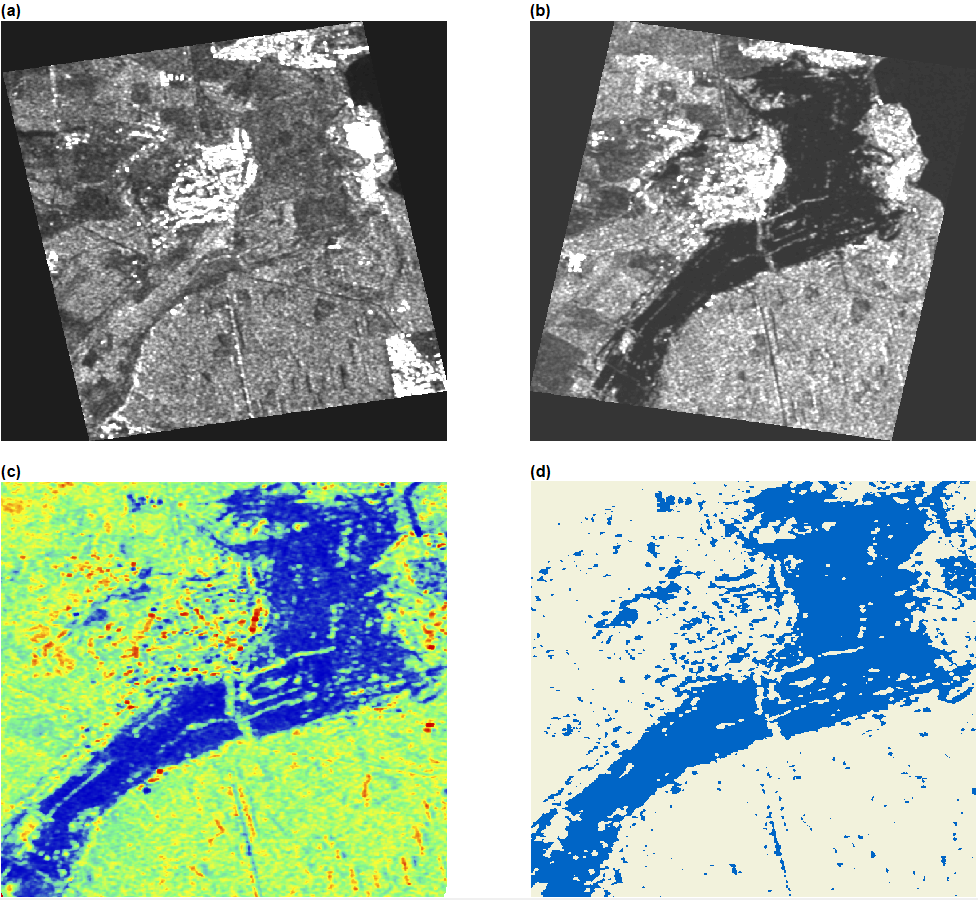
\includegraphics[width=\textwidth]{Bilder/prozess.png}
    \caption{Beispielhafte Prozessierungsergebnisse (a) kalibrierte überflutungsfreie Referenzaufnahme (b) kalibrierte Aufnahme des Überschwemmungsereignisses (c) NDSI  (d) binäre Überschwemmungsmaske (eigene Darstellung)}
    \label{pre_post_ndsi}
\end{figure}


\subsection{Zusätzliche Funktionalitäten}
\subsubsection{Coverage Endpoint} 
Der nicht im Standard definierte Coverage Endpoint kann über den nachstehenden URL mit der HTTP-Get Methode erreicht werden. 
\begin{center}
\begin{BVerbatim}
    http://HOST:PORT/coverage?f=<MEDIA-TYPE>
\end{BVerbatim}
\end{center}
Als Ressource liefert er eine Übersicht aller Sentinel-1 Datensätze, welche persistent gespeichert sind. 
Jobs, welche auf diese Datensätze zugreifen, können schneller abgearbeitet werden, da ein zeitaufwendiges Herunterladen entfällt. 
Die Coverage Ressource kann nur mit der HTTP-Get Methode angefragt werden und steht in den Media-Types \verb|text/html| und \verb|application/json|
zur Verfügung. Dieser kann mit dem Parameter \verb|f| spezifiziert werden.

Eingehende Requests werden zunächst auf die verwendete HTTP-Methode überprüft. Nicht unterstützte HTTP-Methoden werden 
mit Responses mit dem HTTP-Statuscode 405 beantwortet. Spezifiziert der Parameter \verb|f| nicht unterstützte Media-Types, so wird ein Response mit dem 
HTTP-Statuscode 406 versandt. 

Nach Eingang eines gültigen Requests werden zunächst alle \verb|.kml|-Dateien aus dem \emph{Coverage}-Verzeichnis geladen. Aus diesen werden der Produktname, das Aufnahmedatum 
sowie die BBox extrahiert. Diese Informationen werden in Arrays gespeichert. Aus diesen werden entweder direkt Response-Objekte erzeugt oder zusammen mit der 
\verb|coverage.html| dem Renderer übergeben. Die Response-Objekte werden mit dem HTTP-Statuscode 200 sowie dem Headern \verb|link| und \verb|resource| versandt. 
Der \verb|resource|-Header erhält den Wert \verb|coverage|. Fehler resultieren in Responses mit dem HTTP-Statuscode 500. 

Sollen zusätzliche Datensätze einer Region für einen bestimmten Zeitraum persistent in der Anwendung gespeichert werden, so können diese über das 
Copernicus Open Access Hub bezogen werden. Die Datensätze müssen anschließend im \emph{Data}-Verzeichnis abgelegt werden. Teil eines jeden Sentinel-1 Datensatzes 
ist eine \verb|.kml|-Datei. Diese muss im \emph{Coverages}-Verzeichnis  abgelegt werden. Von Prozessen heruntergeladene Datensätze werden automatisch persistent und 
für die Anwendung nutzbar gespeichert (siehe Anhang \ref{PseudocodeCoverage}) \cite{code}. 

\subsubsection{Download Endpoint}
Um das Herunterladen von großen Bilddaten über einen URL zu erlauben, wurde die prototypische Implementierung um den Download Endpoint ergänzt.
Die Verknüpfungen können auch Teil der Prozessierungergebnisse sein, wenn als Response-Typ \verb|document| spezifiziert wurde. 
Bestimmte Dateien können unter dem nachstehenden URL unter Verwendung der HTTP-Methode Get heruntergeladen werden.

\begin{center}
\begin{BVerbatim}
    http://HOST:PORT/download/<jobID>/<requestedFile>
\end{BVerbatim}
\end{center}

Nach Überprüfung der verwendeten HTTP-Methode, wobei eine nicht unterstützte HTTP-Methode in einem Response mit dem HTTP-Statuscode 405 mündet, wird die Existenz des 
spezifizierten Jobs sichergestellt. Existiert dieser nicht, wird eine \verb|no-such-job|-Exception mit dem HTTP-Statuscode 404 versandt.  
Andernfalls werden die \verb|status.json| und \verb|job.json| aus dem \emph{Job}-Verzeichnis geladen. Der Download-Endpoint stellt in der prototypischen 
Implementierung nur die aus dem \verb|FloodMonitoring|-Prozess erzeugten Bilddaten zum Download bereit. Ist der spezifizierte Job eine Instanz des \verb|Echo|-Prozesses 
wird ein Response mit dem HTTP-Statuscode 501 versandt. Es können die \verb|bin.tif| oder die \verb|ndsi.tif| zum herunterladen angefragt werden. Ist eine der beiden Dateien 
durch den \verb|requestedFile|-Parameter spezifiziert, wird die entsprechende Datei mit dem HTTP-Statuscode 200 versandt. Werden andere Dateien durch den Request 
spezifiziert, wird eine \verb|no-such-file|-Exception mit dem HTTP-Statuscode 404 versandt. Responses mit dem HTTP-Statuscode 500 sind das Resultat von Fehlern im 
Programmablauf (siehe Anhang \ref{PseudocodeDownload}) \cite{code}. 

\subsubsection{Test Suit}
Um die Funktionen der API und seine Standardkonformität testen zu können, wurde ein Unit-Test oder test Suit aus dem im Standard beschriebenen Abstract Test Suit abgeleitet und 
implementiert. Zu bemerken ist dabei, dass der prototypische implementierte Test-Suit lediglich einige maschinentestbare Testfälle abdeckt. 
Werden nun Änderungen am Programm vorgenommen, kann mit der Ausführung dieses Test-Suits einfach die Funktionalität und Stabilität der API überprüft werden. 
Bisher sind 35 der 82 Testfälle von der prototypischen Implementierung abgedeckt.

